\documentclass[11pt]{article}
\usepackage[top=2.5cm, bottom=2.5cm, left=2cm, right=2cm]{geometry}
\usepackage[utf8]{inputenc}
\usepackage[icelandic]{babel}
\usepackage[T1]{fontenc}
\usepackage[sc]{mathpazo}
\usepackage[parfill]{parskip}
\usepackage{booktabs}
\usepackage{amsmath}
\usepackage{color}
\usepackage{graphicx}
\usepackage{wrapfig}
\usepackage{subcaption}
\usepackage{minted}
\usepackage{multicol}
\usepackage{lipsum}
\usepackage[pdftex,bookmarks=true,colorlinks=true,linkcolor=blue,urlcolor=blue, citecolor=blue]{hyperref}
\usepackage[all]{hypcap}

\hyphenpenalty=9000

\newcommand{\matlab}[1]{\inputminted[linenos, frame=lines, label=#1, fontsize=\small]{matlab}{#1}}
\renewcommand{\listingscaption}{Kóði}

% One-column environment definitons for multicol - not floating!
\makeatletter
\newenvironment{tableonecolumn}{\begin{minipage}{\linewidth}\begin{center}\def\@captype{table}}{\end{center}\end{minipage}}

\newenvironment{figureonecolumn}{\begin{minipage}{\linewidth}\begin{center}\def\@captype{figure}}{\end{center}\end{minipage}}
\makeatother

\title{Framleiðsla á humulene í Saccharomyces cerevisiae}
\author{Eiríkur Ernir Þorsteinsson \and Jónas Tryggvi Stefánsson}
\date{}

\begin{document}

\maketitle

\setlength{\columnsep}{1cm}

\begin{abstract}
\lipsum[150]
\end{abstract}

\vspace{1cm}
\begin{multicols}{2}

% Myndir verða mikilvægar, fá 2-4
% Byrja á myndunum!
% Hugmynd: Flæðirit yfir virkni reikniritsins
\section{Inngangur}
Áfengi drykkurinn bjór ætti að vera flestum lesendum kunnugur. Hefðbundinn bjór er myndaður með gerjun á vatnsblönduðu korni og bragðbættur með humlum.

Humlar eru dýrt hráefni sem erfitt er að rækta á mörgum svæðum heimsins og hrörna hratt við geymslu. Þetta gefur ástæðu til að athuga hvort að hægt sé að minnka það magn humla sem bjórgerðin þarf með efnaviðbótum.

Humulene er eitt mikilvægra efnasambanda í lykt og bragði bjórs \cite{howard1957evaluation}. Lagt er upp með athuga reikningslegar forsendur fyrir því að nota erfðabreyttan gersvepp til að framleiða humulene, en þó nokkur fordæmi eru fyrir því að erfðabreyta gersveppum til nota í matvælaiðnaði \cite{dequin2001potential}.

Fyrirsjáanlegar eru tvær aðalleiðir til að hagnýta framleiðslu á humulene í gersvepp. Fyrri leiðin er að nota erfðabreyttan gersvepp til að gerja bjór í annars hefðbundnu bjórgerðarferli. Seinni leiðin er að besta framleiðslu á hreinu humulene, sem síðan væri einangrað. 

Báðar hagnýtingarleiðir verða hér kannaðar með aðstoð línulegra bestunarlíkana, en línuleg bestunarlíkön hafa verið notuð með góðum árangri til spá fyrir um möguleg efnaskiptaferli í örverum \cite{banga2008optimization,edwards2001silico}.
\section{Aðferð}
% Fyrsti textinn sem er skrifaður
% Byrja á undirtitlum
% Mikilvægt að strúktúra málsgreinarnar vel
% Mikilvægt að tengja 
Báðar aðferðir byggjast á greiningu á líkani af gersveppnum.
\subsection{Líkan}
Notast var við Yeast 7 líkanið af gersvepp (\emph{Saccharomyces cerevisiae}), sem sótt var af vefsíðunni \url{http://yeast.sourceforge.net/} og þýtt yfir á Matlab-form sem nýtilegt er með Cobra-pakkanum af Steini Guðmundssyni. Líkanið var valið vegna þess að það er umfangsmikið (m.t.t. fjölda gena og efnahvarfa), með lágt hlutfall blokkaðra efnahvarfa og lágt hlutfall dead-end efna. Önnur líkön gefa betri niðurstöður í sérhæfðum aðstæðum, en þessir eiginleikar Yeast 7 þóttu líklegir til að stuðla að nothæfum niðurstöðum í fyrstu hermunum \cite{heavner2015comparative}.

\subsubsection{Viðbætur á líkani}
Þekkt ensím, (2E,6E)-farnesyl-diphosphate diphosphate-lyase, myndar humulene út frá farnesyl-diphosphate \cite[KEGG: R08373]{Kanehisa01012000}. Farnesyl-diphosphate finnst í terpenoid lífefnasmíðaferlinu \cite[KEGG: rn00900]{Kanehisa01012000}, en bestun á því efnaferli hefur fengið nokkra athygli \cite{BIT:BIT21216,misawa2011pathway,asadollahi2008production}.

Tveimur grundvallar-efnahvörfum var bætt við líkanið til að framleiða humulene úr farnesyl-diphosphate.
Um er að ræða efnahvarf sem framleiðir humulene úr farnesyl-diphosphate annars vegar og exchange-hvarf fyrir humulene-ið hins vegar. Sjá mynd \ref{fig:pathway}

\begin{figureonecolumn}
\caption[Viðbætur við Yeast 7]{Efnahvörf sem bætt var við Yeast 7 líkanið.}
\label{fig:pathway}
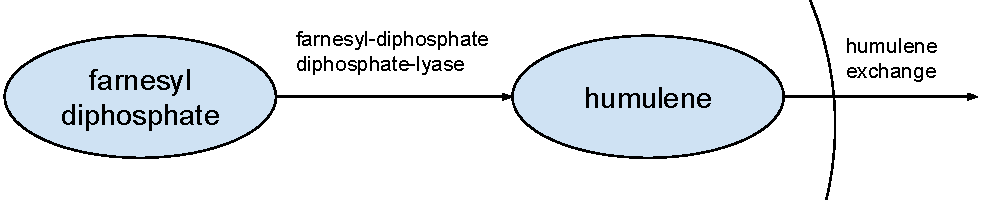
\includegraphics[width=\linewidth]{Pics/HumuleneAddition}
\end{figureonecolumn}
\subsection{Framleiðsla í hefðbundnu gerjunarferli}
\label{sec:hefdbundid}
\subsubsection{Kolefnisgjafar og gefin skilyrði}
Gerjanlegu sykrurnar í virti eru frúktósi, glúkósi, súkrósi, maltósi og maltótríósi. Þar vega mest hlutverk maltósa, frúktósa og maltótríósa. Maltótríósi er ekki til staðar í Yeast 7 líkaninu og hlutverk annarra kolefnisgjafa er óverulegt, svo til einföldunar voru einungis maltósi og glúkósi tekin til skoðunar. Valin hlutföll eru 1 hlutur glúkósa á móti 2 hlutum maltósa, sem er nálægt meðalhlutföllum þeirra í virti \cite{otter1967determination}. 

Í bjórgerð fer gerjun fram við að mestu leyti loftfirrtar aðstæður. \emph{S. cerevisiae} getur vaxið við slík skilyrði \cite{ishtar2007factors}, en líkanið nær ekki til þeirra.
\subsubsection{Markfall}
Þar sem framleiða á vöru til neyslu er nauðsynlegt að stýra framleiðslu á fleiri efnum en einungis humulene. Mikilvæg efni í bjór \cite{dequin2001potential} sem tekin voru til athugunar eru:
\begin{itemize}
 \item etanól
 \item ísóamýl acetat, ábyrgt fyrir ``bananalykt'' af ýmsum gerðum bjórs
 \item glýseról, veitir sætutilfinningu
 \item þvagefni, sem ólykt er af og þarf að lágmarka
\end{itemize}
Markfall var smíðað sem tekur tillit til þessara efna. 

Æskilegu efnunum var úthlutað stuðlum sem jafna forgang þeirra m.t.t. fjölda kolefnisfrumeinda í efnunum, til að koma í veg fyrir að Cobra úthluti efnahvörfum sem seyta efnum með fáum kolefnisfrumeindum óeðlilega miklu flæði. ``Rétt'' gildi á þessum efnum myndi fara eftir gerð bjórsins sem framleiða ætti. Þetta er gert í kóðadæmi \ref{code:addTargetMetabolite}.

\subsection{OptStrain}
\label{sec:optstrain}
\begin{figure*}
\caption[OptStrain reikniritið]{Skref OptStrain reikniritsins sem lýst er í \ref{sec:optstrain}. Sjá sérstakar viðbætur á mynd \ref{fig:pathway}}
\label{fig:flaedirit}
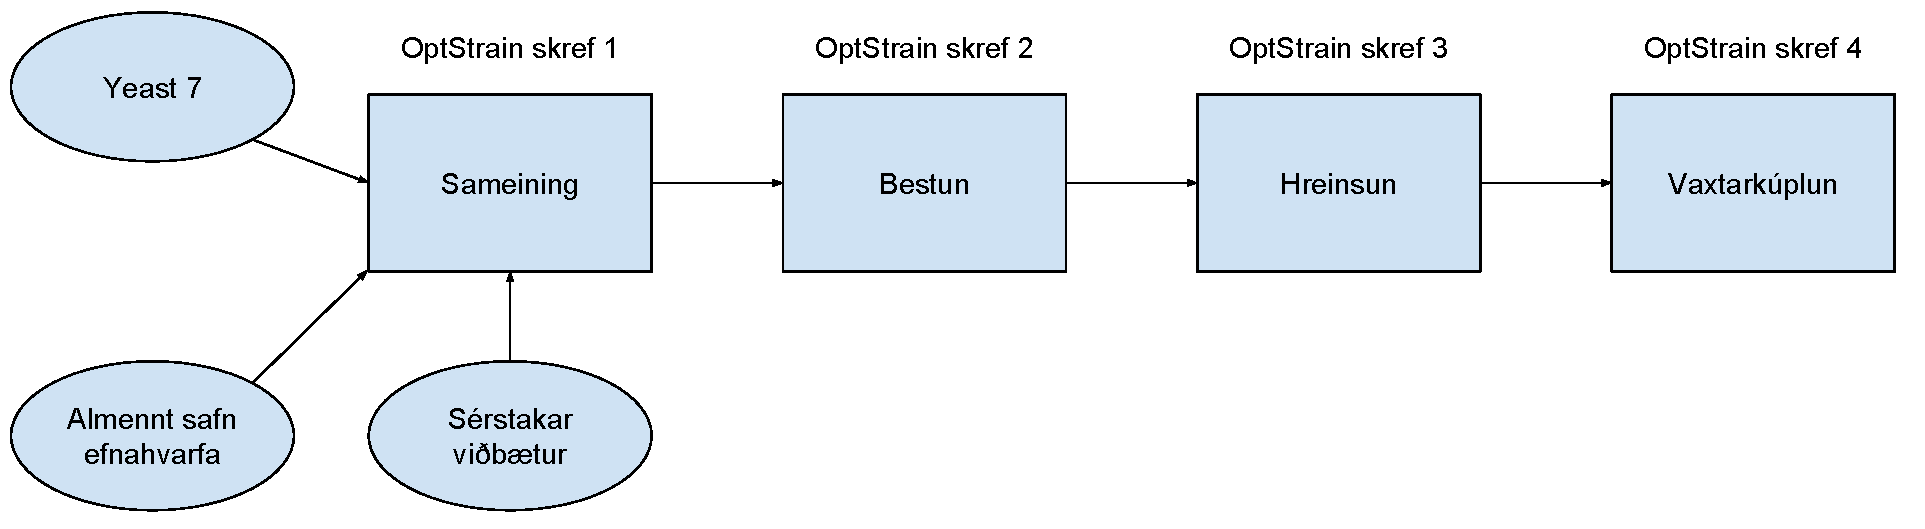
\includegraphics[width=\linewidth]{Pics/OptStrainOverview}
\end{figure*}
\subsubsection{Almenn lýsing}
\subsubsection{Útfærsla}

\section{Niðurstöður}

% Undirtitlar hér líka

\begin{figureonecolumn}
\caption{Hámarksflæði með og án bestunar á humulene-framleiðslu}
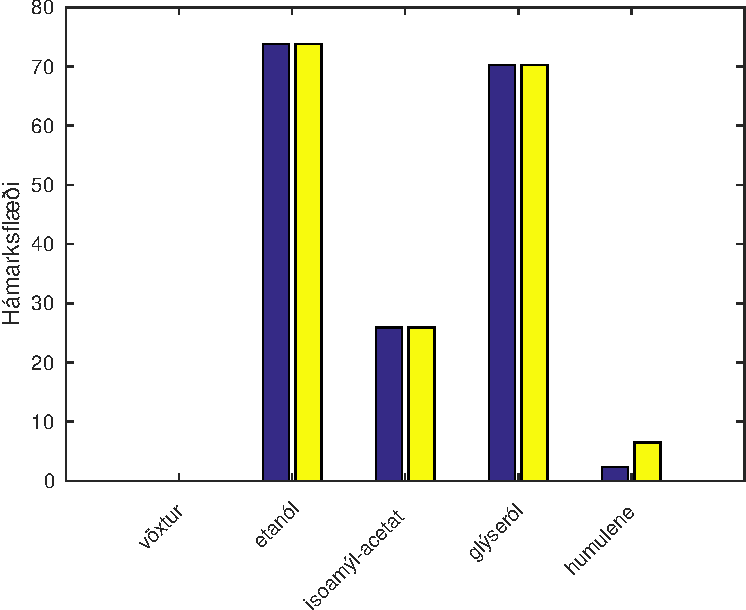
\includegraphics[width=\linewidth]{Pics/BrewingMetMaxFlow}
\end{figureonecolumn}

\begin{figureonecolumn}
\caption{Áhrif humulene-framleiðslu á markfallsgildi}
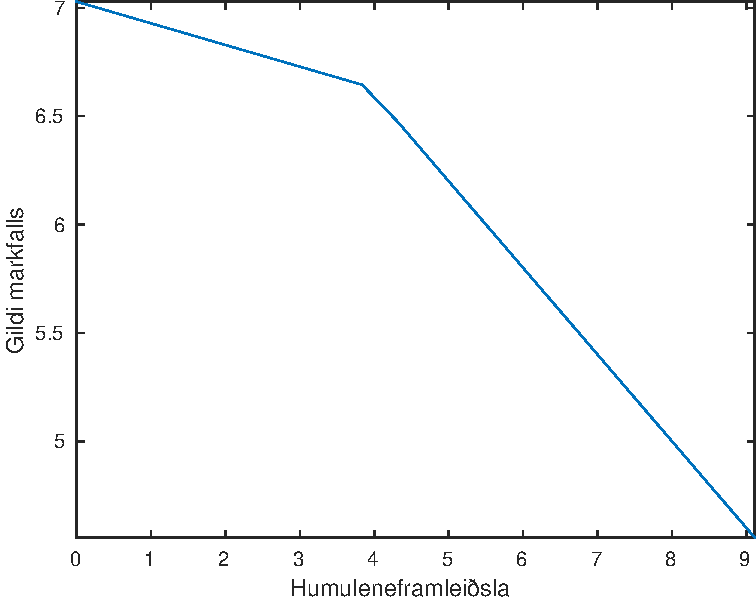
\includegraphics[width=\linewidth]{Pics/BrewingRobustnessAnalysis}
\end{figureonecolumn}

\section{Samantekt}
% Byrjar oftast eins: Here we set out to...

% \paragraph{Samantekt á niðurstöðum}
% \paragraph{Hvernig falla niðurstöðurnar að öðrum þekktum niðurstöðum}
% Ræða hvern undirtitil í niðurstöðu-hlutanum sérstaklega
% Aftur samantekt á síðustu málsgreinum, summary of impact

Í framhaldinu: Skoða Myrcene \cite[KEGG: C06074]{Kanehisa01012000}, sem er mögulega mikilvægasta sesquiterpene-ið þegar kemur að lykt bjórs \cite{guadagni1966odour}.

%%%%%%%%%%%%%%
% HEIMILDASKRÁ
%%%%%%%%%%%%%%
\bibliographystyle{plain}
\bibliography{bioinfo.bib}

\end{multicols}

%%%%%%%%%%%%%%
% VIÐAUKI
%%%%%%%%%%%%%%

\clearpage
\appendix
\section{Kóði}
\begin{listing}[H]
\caption[addTargetMetabolite]{Fall sem endurskilgreinir gefið módel, í þessu tilfelli er humulene-framleiðslu bætt við}
\label{code:addTargetMetabolite}
\matlab{../addTargetMetabolite.m}
%\inputminted[linenos, frame=lines, label=addTargetMetabolite.m, fontsize=\small]{matlab}{../addTargetMetabolite.m}
\end{listing}

\end{document}